\chapter{Motor}
\section{Stappenmotor}
Een stappenmotor(zie figuur~\ref{fig:stappenmotor}) werkt door stroom op bijvoorbeeld: fase 1,3,5 en 7 te plaatsen terwijl op fase 2,4,6 en 8 grond staat om de as 45 graden te laten draaien. Vervolgens zet je grond op waar stroom op heeft gezeten en vise versa.

\section{Direct current motor}
De DC motor(zie figuur~\ref{fig:dc_motor}) werkt door stroom te geven op het moment dat de motor de evenwichtssituatie nadert. Bij een stilstaande motor wordt er een puls gegeven om de motor een kwartslag te draaien waarna de ingebouwde magneten de motor verder draaien vanwege tegenwerkende polen. Als de motor weer richting de evenwichtssituatie gaat wordt er weer stroom gezet op de motor om hem weer uit deze positie te halen. Door deze herhaling blijft de motor draaien
\\
\begin{figure}[ht]
\begin{subfigure}{0.6\textwidth}
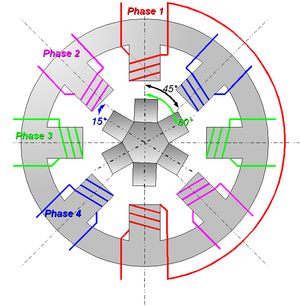
\includegraphics[height=5cm]{src/stepper_motor_schematic} 
\caption{Stappenmotor}
\label{fig:stappenmotor}
\end{subfigure}
\hfill
\begin{subfigure}{0.4\textwidth}
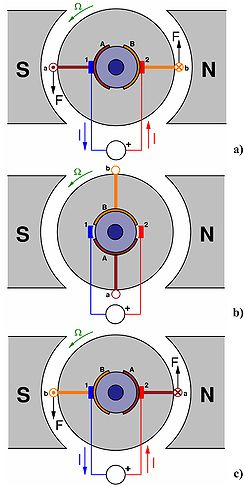
\includegraphics[height=5cm]{src/dc_motor_schematic}
\caption{DC motor}
\label{fig:dc_motor}
\end{subfigure}
\caption{Schematische weergave van de motoren}
\label{fig:motors}
\end{figure}

\section{Voor- en nadelen}
\begin{center}
\begin{tabular}{l|c|c} 
& Stappenmotor & DC motor \\
\hline
Nauwkeurig & \cmark & \xmark \\
\hline
Krachtig bij gelijk wattage & \cmark & \xmark \\
\hline
Simpel in gebruik & \xmark & \cmark \\
\hline
Prijs & \euro{12} - \euro{30} & \euro{5} - \euro{20}
\end{tabular}
\end{center}

\section{Advies}
Voor de motor adviseren wij een stappenmotor aan. Dit omdat in combinatie met de spoel(zie \ref{sec:spoel} voor meer informatie) een krachtige motor nodig is. Daarnaast kunnen wij de lift met een lage snelheid laten draaien zonder kracht te verliezen.